To assess the reliability of CCM, we began by simulating the dynamics of two strains with stochastic, seasonally varying transmission rates (Methods).
In large systems, many factors might influence these rates.
In low-dimensional models, these factors are typically represented as process noise.
We consequently varied the level of process noise in our simulations by changing its standard deviation, $\eta$.
We also varied the strength of competition from strain 2 on strain 1 ($\sigma_{12}$); strain 1, in contrast, never affected strain 2 ($\sigma_{21}=0$).
For each level of competition and process noise, we simulated 100 replicates from random initial conditions to stochastic fluctuations around a deterministic attractor.
One thousand years of error-free monthly incidence were output to give CCM the best chance to work.
For each combination of parameters (competition strength $\sigma_{12}$ and process noise $\eta$), we examined whether strain interactions were correctly inferred.
When $\sigma_{12} >0$, strain 2 should be inferred to ``drive'' (influence) strain 1. 
Because $\sigma_{21}=0$, strain 1 should never be inferred to drive strain 2. 

To detect interactions, for each individual time series, we identified the delay-embeddings (Fig. \ref{fig:conceptual}A) and applied one of two causality criteria using the reconstructed attractors (Fig. \ref{fig:conceptual}B,C and Methods). 
Both criteria are based on the cross-map correlation $\rho$, which is the correlation between reconstructed values of $\hat{Y}$ and actual values of $Y$, given the reconstructed attractor of $X$.
We use $p < 0.05$ to identify significant differences in these correlations because we are interested in situations in which the null hypothesis of no change in correlation, and thus no interaction, is rejected.
Criterion 1 \cite{Sugihara2012, Clark2015} measures whether the cross-map correlation increases as the number of observations of the putatively driven variable grows (Fig. \ref{fig:conceptual}B).
We refer to this as the cross-map increase criterion.
Criterion 2 \cite{Ye2015} infers a causal interaction if the maximum cross-correlation of the putative driver is positive and occurs in the past (i.e., at a negative temporal lag; Fig. \ref{fig:conceptual}C).
We refer to this as the negative cross-map lag criterion.
For simplicity, we start with Criterion 1.


\subsection*{Sensitivity to periodicity}

Criterion 1, which requires a significant increase in cross-map correlation $\rho$ with observation library size $L$, frequently detected interactions that did not exist.
In all cases where strain 2 had no effect on strain 1, CCM always incorrectly inferred an influence (Fig.~\ref{fig:univar_monthly_hm_tmp}A).
Although strain 1 never influenced strain 2, it was often predicted to (Fig.~\ref{fig:univar_monthly_hm_tmp}A). 
Sample time series suggested a strong correlation between synchronous oscillations and the appearance of bidirectional interactions (Fig.~\ref{fig:univar_monthly_hm_tmp}B).
In contrast, when strain 2 appeared to drive strain 1 but not vice-versa ($\sigma_{12}=0$ and $\eta=0.05$), strain 1 often oscillated with a period that was an integer multiple of the other strain's (Fig.~\ref{fig:univar_monthly_hm_tmp}C).
Thus, as expected, strongly synchronized dynamics prevented separation of the variables.
Additionally, the resemblance of strain 2 to the seasonal driver led to false positives even when the strains were independent and strain 1 oscillated at a different frequency.

\begin{figure}
\begin{center}
  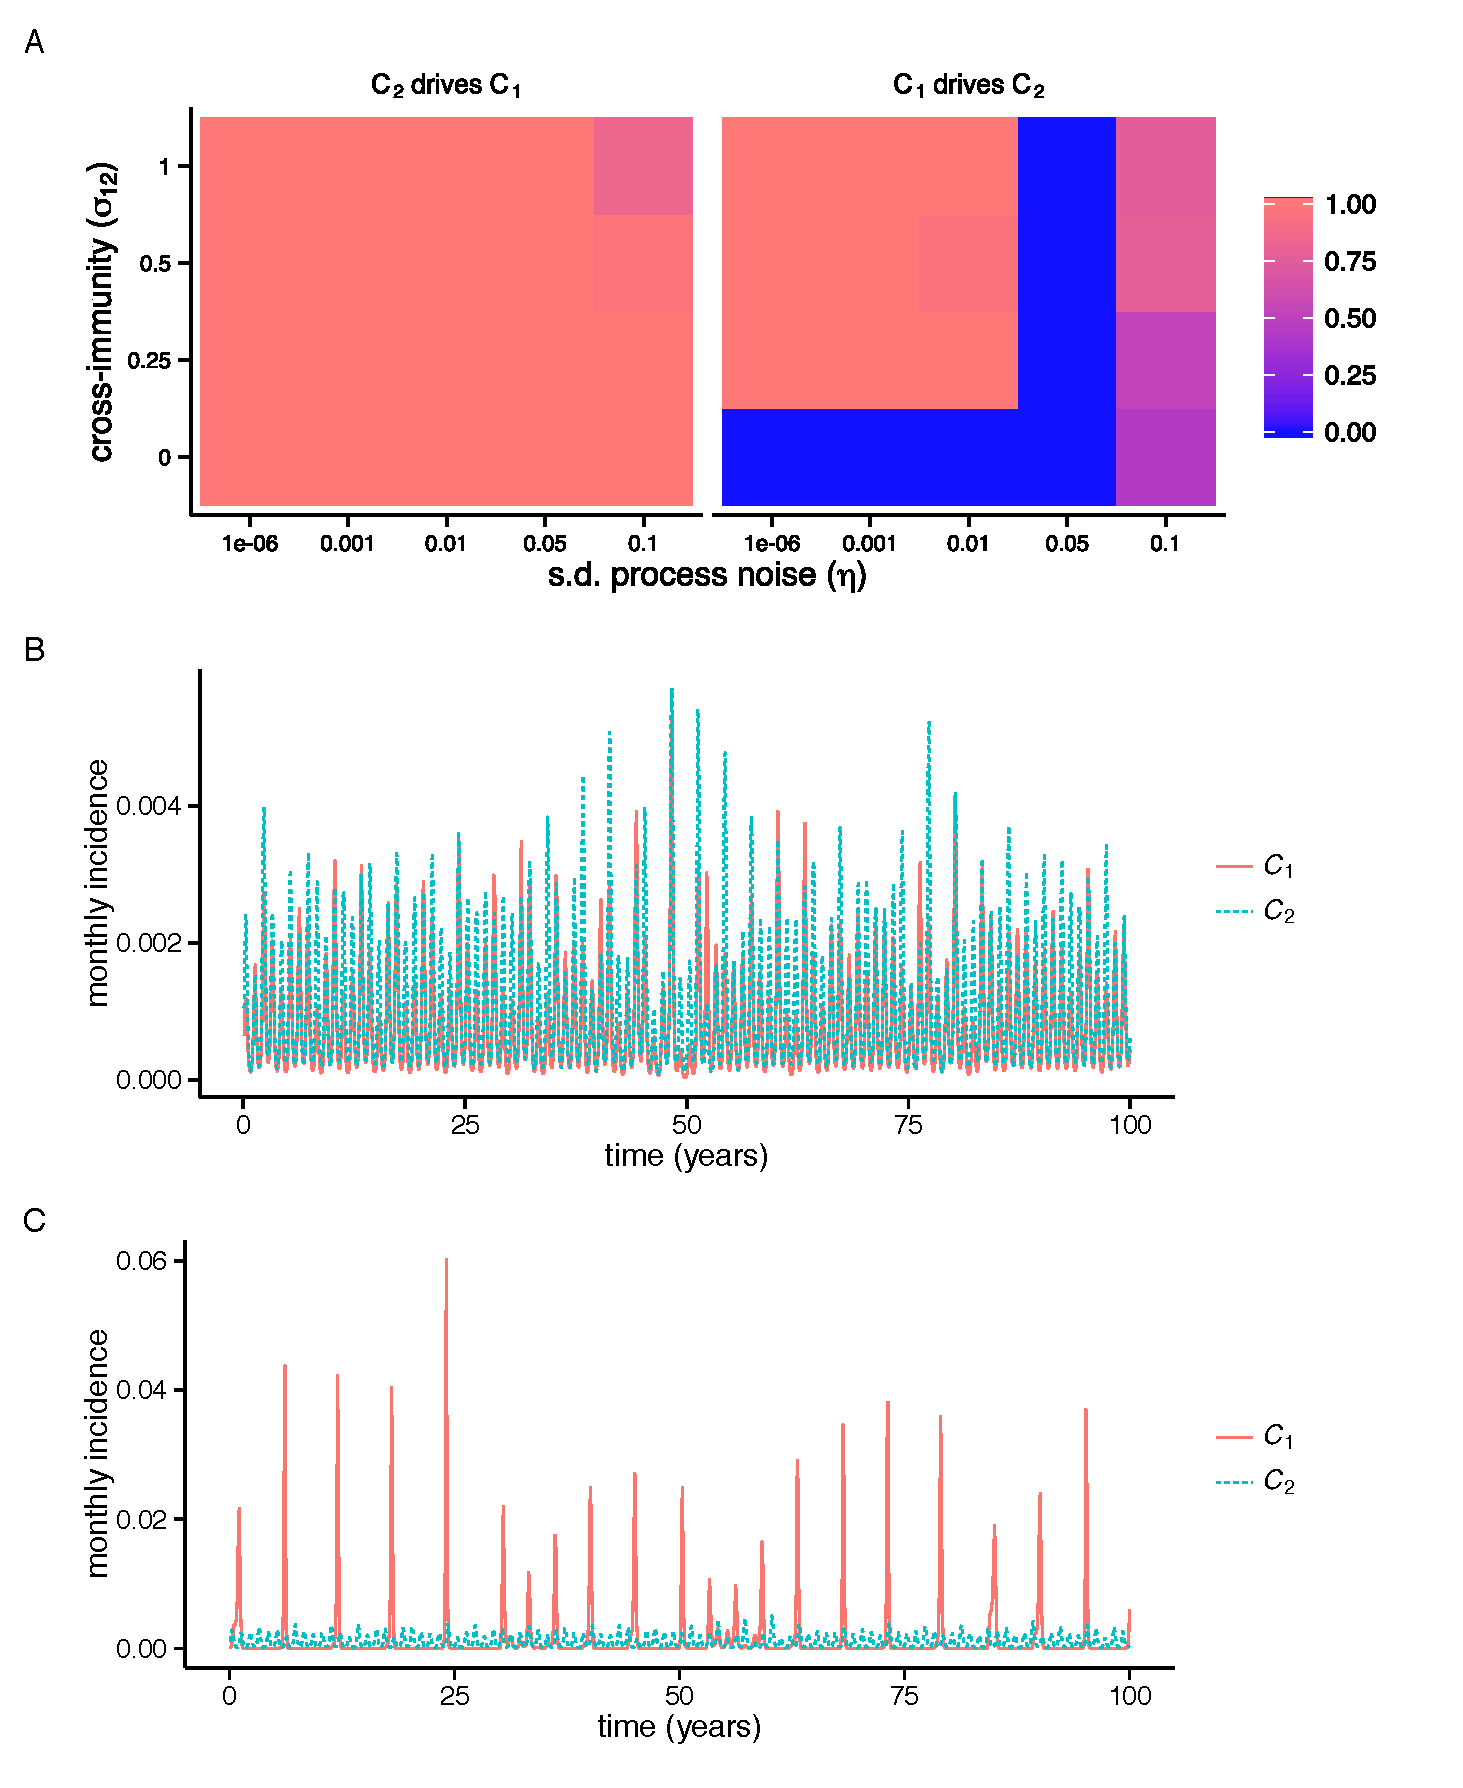
\includegraphics[width=6in]{dataflow/out/fig_detect_increase/fig_detect_increase.pdf}
  \end{center}
  \caption{\textbf{Interactions detected as a function of process noise and the strength of interaction ($C_2 \rightarrow C_1$) and representative time series}. (A) Heat maps show the fraction of 100 replicates significant for each inferred interaction for different parameter combinations. A significant increase in cross-map correlation $\rho$ with library length $L$ indicated a causal interaction. The time series consisted of 1000 years of monthly data. (B) Representative 25-year sample of the time series for which mutual interactions were inferred ($\sigma_{12}=0.25, \eta=0.01$). (C) Representative sample of the time series for which $C_2$ is inferred to drive $C_1$ but not vice-versa ($\sigma_{12}=0.25, \eta=0.05$).  \label{fig:univar_monthly_hm_tmp}} 
\end{figure}

The sensitivity of the method to periodicity persisted despite transformations of the data and changes to the  driver. 
One possible solution to reducing seasonal effects, sampling annual rather than monthly incidence, reduced the overall rate of false positives but also failed to detect some interactions (Fig.~\ref{fig:detect_diffdata}A).
Furthermore, when the effects of strain 2 on 1 were strongest, the reverse interaction was more often inferred.
Sampling the prevalence at annual intervals gave similar results (Fig.~\ref{fig:detect_diffdata}B), and first-differencing the data did not qualitatively change outcomes (Fig.~\ref{fig:detect_diffdata}C).
The method yielded incorrect results even without seasonal forcing ($\epsilon=0$) because of noise-induced oscillations (Fig.~\ref{fig:detect_diffdata}D).
In all of these cases, the presence of shared periods between the strains correlated strongly and significantly with the rate of detecting a false interaction (Fig.~\ref{fig:max_crossspec_tmp}).

Because cross-map skill should depend on the quality of the reconstructed attractor, we investigated performance under other methods of constructing the attractors of the two strains (Methods).
Nonuniform embedding methods allow the time delays to occur at irregular intervals, $\tau_1, \tau_2, ... \tau_{E-1}$, which may provide a more accurate reconstruction.
Alternative reconstruction methods, including nonuniform embedding \cite{Nichkawde2013, Uzal2011}, random projection \cite{Tajima2015}, and maximizing the cross-map (rather than univariate) correlation failed to fix the problem (Fig.~\ref{fig:detect_diffembed}).

\begin{figure}
\begin{center}
  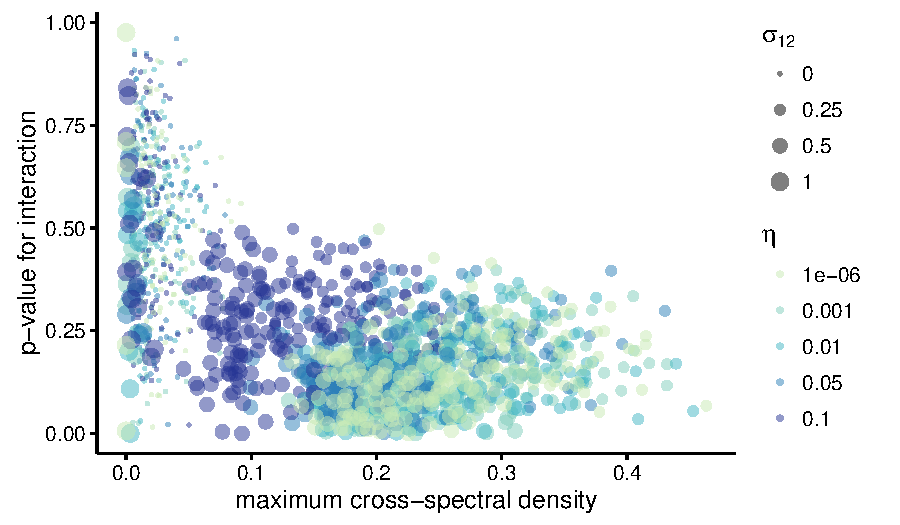
\includegraphics[width=6in]{dataflow/out/fig_spectra/fig_spectra.pdf}
  \end{center}
  \caption{\textbf{Shared frequency spectra predict probability of inferred interaction}. Points show the maximum cross-spectral densities of strains 1 and 2 plotted against the p-values for $C_1 \rightarrow C_2$ for 1000 years of annual data. In all replicates, $C_1$ never actually drives $C_2$. Point color indicates the strength of $C_2 \rightarrow C_1$ ($\sigma_{12}$), and point size indicates the standard deviation of the process noise ($\eta$) on transmission rates. \label{fig:max_crossspec_tmp}} 
\end{figure}

Criterion 2, which infers that $Y$ drives $X$ if there is a positive cross-map correlation that is maximized at a negative cross-map lag, performed relatively well (Fig.~\ref{fig:univar_monthly_lag_seas_diff_tmp}).
Fewer false positives were detected, although the method missed some weak extant interactions ($\sigma_{12}=0.25$) and interactions in noisy systems ($\eta=0.05, 0.1$).
Results for annual data were similar (Fig.~\ref{fig:detect_diffdata_lag}A).
Requiring that $\rho$ be not only positive but also increasing barely affected performance (Fig.~\ref{fig:detect_diffdata_lag}B). 

\begin{figure}
\begin{center}
  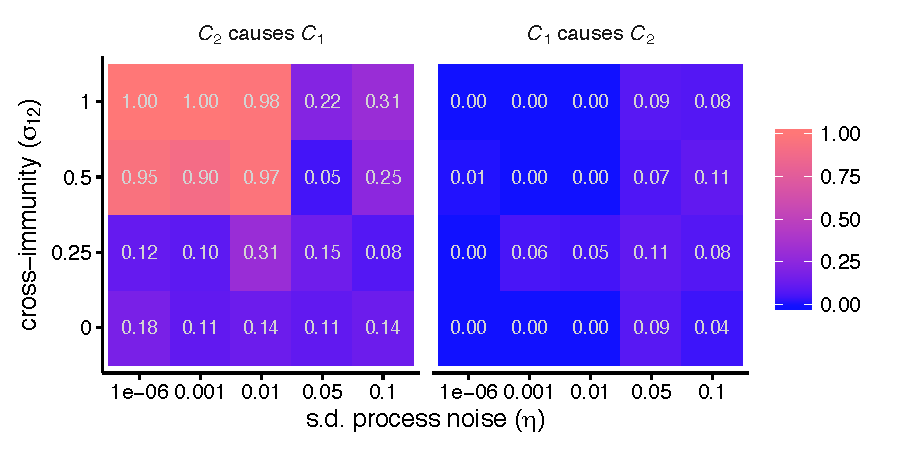
\includegraphics[width=6in]{dataflow/out/fig_detect_lag/fig_detect_lag.pdf}
  \end{center}
  \caption{\textbf{Interactions detected as a function of process noise and the strength of interaction ($C_2 \rightarrow C_1$) and representative time series}. Heat maps show the fraction of 100 replicates significant for each inferred interaction for different parameter combinations. A maximum, positive cross-map correlation $\rho$ at a negative lag indicated a causal interaction. Each replicate used 100 years of monthly incidence. \label{fig:univar_monthly_lag_seas_diff_tmp}} 
\end{figure}

\subsection*{Limits to identifiability}

If two variables $X$ and $Y$ share the same driver but do not interact, if the driving is strong enough, $X$ may resemble the driver so closely that $X$ appears to drive $Y$.
In a similar vein, when the two strains in our system have identical transmission rates ($\beta_1= \beta_2$) and one strongly drives the other ($\sigma_{12}=1$), the direction of the interaction cannot be detected when the dynamics are nearly deterministic ($\eta=10^{-6}$) (Fig.~\ref{fig:detect_diffdata_lag}C). 
Causal inference in such cases becomes difficult.

To investigate the limits to distinguishing strains that are ecologically similar and do not interact, we varied the correlation of the strain-specific process noise while applying the more conservative of the two criteria for inferring causality (Criterion 2), that the cross-map correlation $\rho$ be positive and peak at a negative lag \cite{Ye2015}.
Process noise can be thought of as a hidden environmental driver that affects both strains simultaneously, and thus the strength of correlation indicates the relative contribution of shared versus strain-specific noise.  
With two identical, independent strains, no seasonal forcing, and low process noise ($\eta=0.01$), the false positive rate depended on correlation strength and the quantity of data.
When using 100 years of monthly incidence, the false positive rate varied non-monotonically with correlation strength, with a minimum (5\%-6\%) at a correlation of 0.75 and its highest values, near 24\%, at correlations of 0 and 1 (Fig.~\ref{fig:detect_corrproc_identical}A).
Using 1000 years of annual incidence reduced false positive rates to 5\%-9\% for imperfectly correlated noise (Fig.~\ref{fig:detect_corrproc_identical}B).
The best performance occurred with 100-year monthly data when cross-map correlation was required to increase with library length (Fig.~\ref{fig:detect_corrproc_identical}C).
Thus, the independence of two strains will generally be detected as long as they experience imperfectly correlated noise. 

We next considered the problem of identifying two ecologically distinct strains ($\beta_1 \neq \beta_2$) when one strain strongly drives the other ($\sigma_{12}=1$) and its dynamics resemble the seasonal driver.
In this case, even with perfectly correlated process noise, correct interactions are consistently inferred (Fig.~\ref{fig:detect_corrproc_distinct}).
Thus, we conclude that the presence of noise, even highly correlated noise, can help distinguish causality between coupled, synchronized variables \cite{Schumacher2015}.
It is more difficult to distinguish non-interacting, dynamically equivalent variables.
In the latter case, noise has inconsistent effects on causal inference, although Criterion 2 may perform much better than Criterion 1.
These results at least hold for ``modest'' noise ($\eta=0.01$): as shown earlier, higher levels hurt performance (Fig.~\ref{fig:univar_monthly_lag_seas_diff_tmp}).


\subsection*{Transient dynamics}
CCM is optimized for dynamics that have converged to a deterministic attractor.
Directional parameter changes in time and large perturbations can prevent effective cross-mapping because the method requires a consistent mapping between system states as well as sufficient coverage of state space by the data.
We evaluated the impact of both of these types of transient dynamics on causal inference, using a simple example of each as proof of principle.

In the first test, we identified two sets of parameter values where CCM was successful under Criterion 2 (intermediate interaction strength, $\sigma_{21} = 0.5$; seasonal forcing, $\epsilon = 0.1$; process noise, $\eta = 0.01$; and transmission rates $\beta_1$ of $0.30$ (Fig.~\ref{fig:betachange}A) and $0.32$ (Fig.~\ref{fig:betachange}B)).
We tested CCM on simulations with the parameter values fixed and then with the transmission rate $\beta_1$ varying linearly over time betwen the two values.
All three tests used 100 years of monthly incidence.
Of 100 replicates, with $\beta_1$ fixed at $0.30$, CCM failed to detect an interaction 5 times, and never falsely detected an absent interaction.
With $\beta1$ fixed at $0.32$, there were 12 false negatives and 1 false positive.
When $\beta_1$ varied from $0.30$ to $0.32$, error rates increased: there were 29 false negatives and 44 false positives.
Transient dynamics due to a linear change in a system parameter can thus lead to incorrect causal inference even when causal inference is successful before and after the change.

\begin{figure}
    \begin{center}
      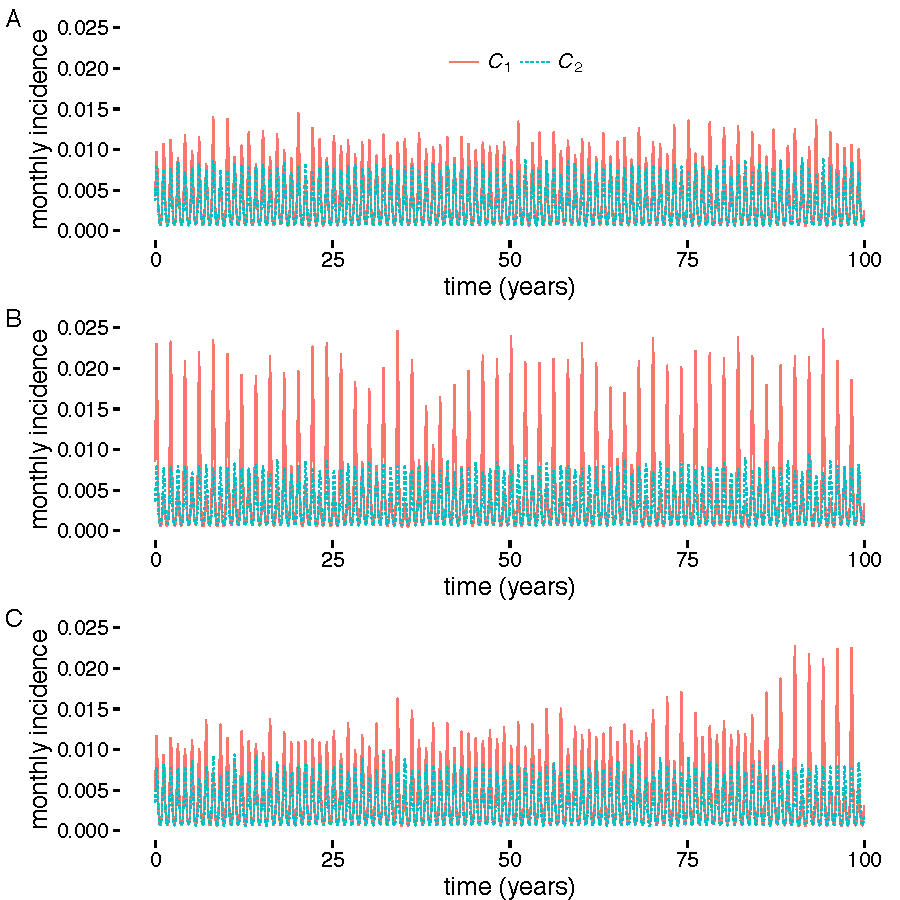
\includegraphics[width=6in]{dataflow/out/fig_betachange/fig_betachange.pdf}
    \end{center}
    \caption{\textbf{Incorrect inference with changing transmission rate.} Example time series for testing transient dynamics. Each time series contained 100 years of monthly incidence data. The transmission rate $\beta_1$ for the driven strain $C_1$ was fixed at $\beta_1 = 0.30$ (A) and $\beta_1 = 0.32$ (B), and varied linearly over time between the two values (C). The transient time series yields high false positive and false negative rates under CCM. Interaction strength was $\sigma_{21} = 0.5$, process noise was $\eta = 0.01$, and seasonal forcing was $\epsilon = 0$. \label{fig:betachange}} 
\end{figure}

In the second test, we began simulations at random initial conditions far from equilibrium and applied CCM to the first 100 years of monthly incidence.
% select count(*) from ccm_lag_tests where neg_pvalue_best <= 0.05 and cause = 'C0'
% select count(*) from ccm_lag_tests where neg_pvalue_best <= 0.05 and cause = 'C1'
When strain 2 weakly drives strain 1 ($\sigma_{12}=0.5$), causal inference is compromised, even when process noise is low ($\eta=0.01$; Fig.~\ref{fig:transient}).
In 100 simulations of this scenario, the correct interaction (strain 2 driving strain 1) was always detected after transients had passed, but it was detected in only 19 of 100 simulations that included transients.
Furthermore, a reverse interaction (strain 1 driving 2) was incorrectly detected in 21 of 100 simulations.
The method thus performed worse than chance in identifying interactions that were present, and it also regularly predicted nonexistent interactions.

\subsection*{Application to childhood infections}

Given the apparent success of CCM under Criterion 2 (negative cross-map lag) with two strains and little noise near the attractor, we investigated whether the method might shed light on the historic dynamics of childhood infections in the pre-vaccine era.
Time series analyses have suggested that historically common childhood pathogens may have competed with or facilitated one another \cite{Mina2015, Rohani2003}.
We obtained the weekly incidence of six reportable infections in New York City from intermittent periods spanning 1906 to 1953 \cite{vanPanhuis2013} (Fig.~\ref{fig:historical_data_tmp}A).
Six of 30 pairwise interactions were significant at the $p<0.05$ level, not correcting for multiple tests (Fig.~\ref{fig:historical_data_tmp}C).
Polio drove mumps and varicella, scarlet fever drove mumps and polio, and varicella and pertussis drove measles. 
Typical cross-map lags occurred at one to three years (Fig.~\ref{fig:cities_corrbylag_nyc_self_uniform}).
The inferred interactions were identical if we required that the cross-map correlation $\rho$ be increasing and not merely positive.

\begin{figure}
\begin{center}
  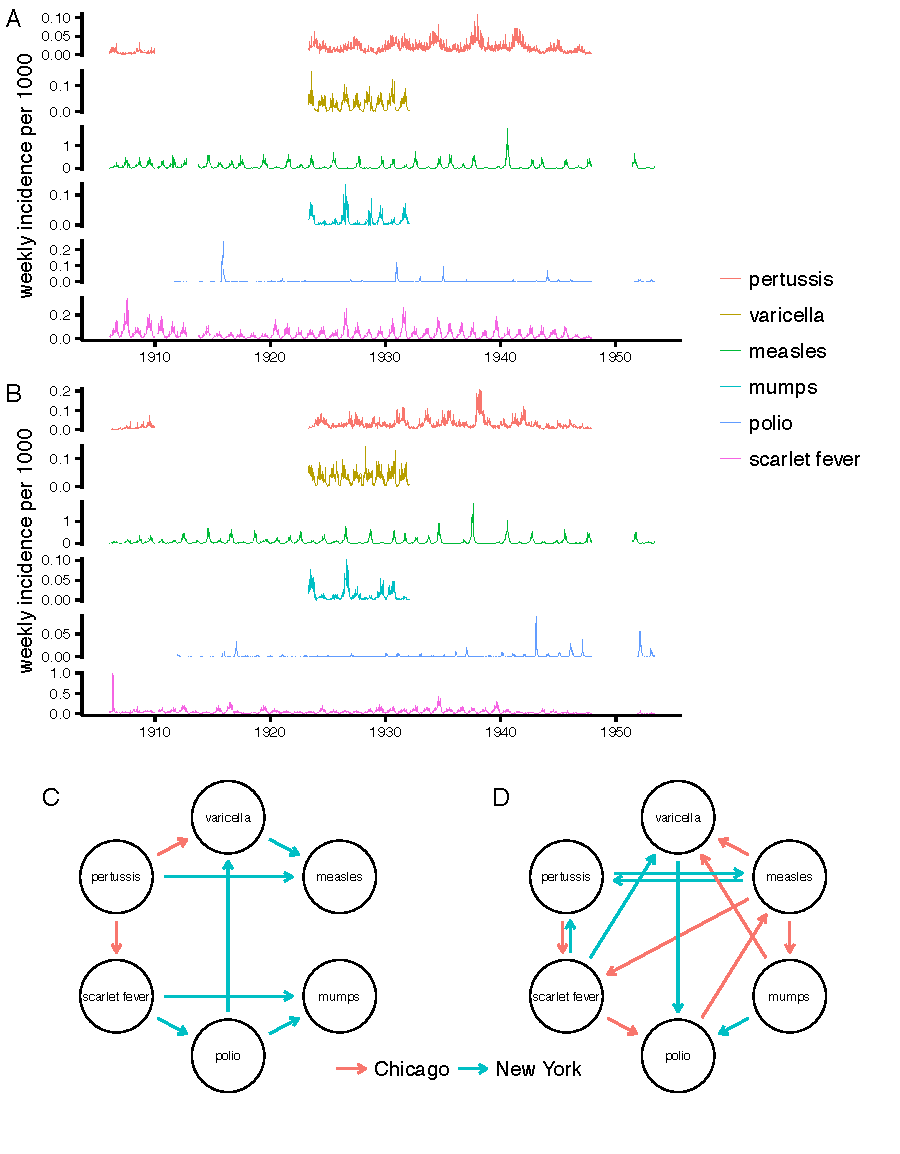
\includegraphics[width=6in]{dataflow/out/fig_cities/fig_cities.pdf}
  \end{center}
    \caption{\textbf{Historical childhood infections in New York City and Chicago and inferred interactions from two reconstruction methods.} Time series show weekly incidence of infections per 1000 inhabitants of New York City (A) and Chicago (B). Delay-embeddings were constructed by maximizing the univariate correlation (C) or through a random projection method (D) Arrows indicate the inferred interactions from the New York (blue) and Chicago (red) time series under Criterion 2 (negative cross-map lag).\label{fig:historical_data_tmp}} 
\end{figure}

Although we specifically chose infectious diseases not subject to major public health interventions in the sampling period, it is possible that the New York data contain noise and transient dynamics.
To the check robustness of the conclusions, we analyzed analogous time series from Chicago from the same period (Fig.~\ref{fig:historical_data_tmp}B).
Completely different interactions appeared (Fig.~\ref{fig:historical_data_tmp}C).
Not correcting for multiple tests, pertussis drove scarlet fever and varicella; accepting marginally significant negative lags ($p=0.055$), polio drove measles.
In these cases, the maximum cross-map correlation $\rho$ was not only positive but also increased at negative lag.
Requiring that $\rho$ only be positive at negative lag, polio also drove pertussis, measles drove mumps and varicella, and mumps drove scarlet fever.
Except in one case, all negative lags occurred at more than one year (Fig.~\ref{fig:cities_corrbylag_chi_self_uniform}).
Thus, no consistent interactions appeared in epidemiological time series of two major, and possibly dynamically coupled, cities.

To investigate the possibility that our method of attractor reconstruction might be unduly sensitive to noise and transient dynamics, we repeated the procedure with a method based on random projections \cite{Tajima2015}.
Once again, no interactions were common to both cities (Fig.~\ref{fig:historical_data_tmp}D).
Furthermore, only one of the original eight interactions from the first reconstruction method reappeared with random projection (two of eight reappeared if disregarding the city), and two interactions changed direction (three if disregarding the city). 
Both reconstruction methods selected similar lags (Figs.~\ref{fig:cities_corrbylag_nyc_cross_projection},~\ref{fig:cities_corrbylag_chi_cross_projection}).
